% ******************************* Thesis Appendix B ********************************
\chapter{\mindphistar requirement in the signal region}
\label{ch:app_dphistar}

As described in chapter~\ref{ch:5}, an event level requirement is made in the
signal region such that all events have \mindphistar > 0.3, in order to remove
any remaining QCD MJ contamination. This appendix outlines some of
the studies to motivate and characterise this requirement.

\section{Motivation}

The hadronic signal region selection criteria are specifically
designed to remove many orders of magnitude of QCD MJ events, in particular
through the use of variables such as \alphat and \mhtmet.
However, despite these strict requirements a small fraction of QCD MC events are
observed to still enter into the pass the selection criteria.

\begin{figure}[h!]
  \centering
  \begin{subfigure}[b]{0.46\textwidth}
    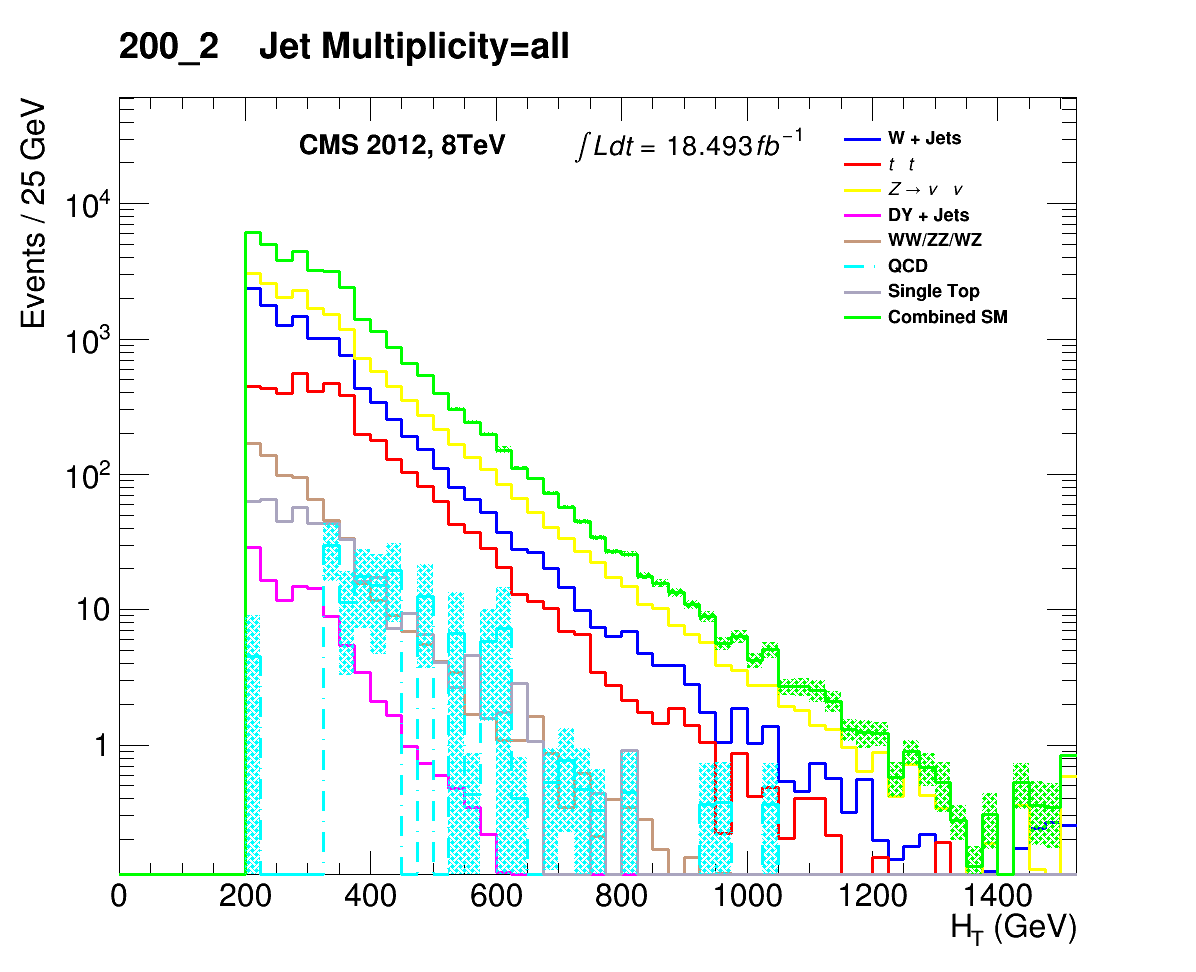
\includegraphics[width=\textwidth]{Figs/datamc/had/qcd/HT_all_200_upwards.png}
    \caption{\HT}
    \label{fig:had_qcd_mc_HT}
  \end{subfigure}
  \begin{subfigure}[b]{0.46\textwidth}
    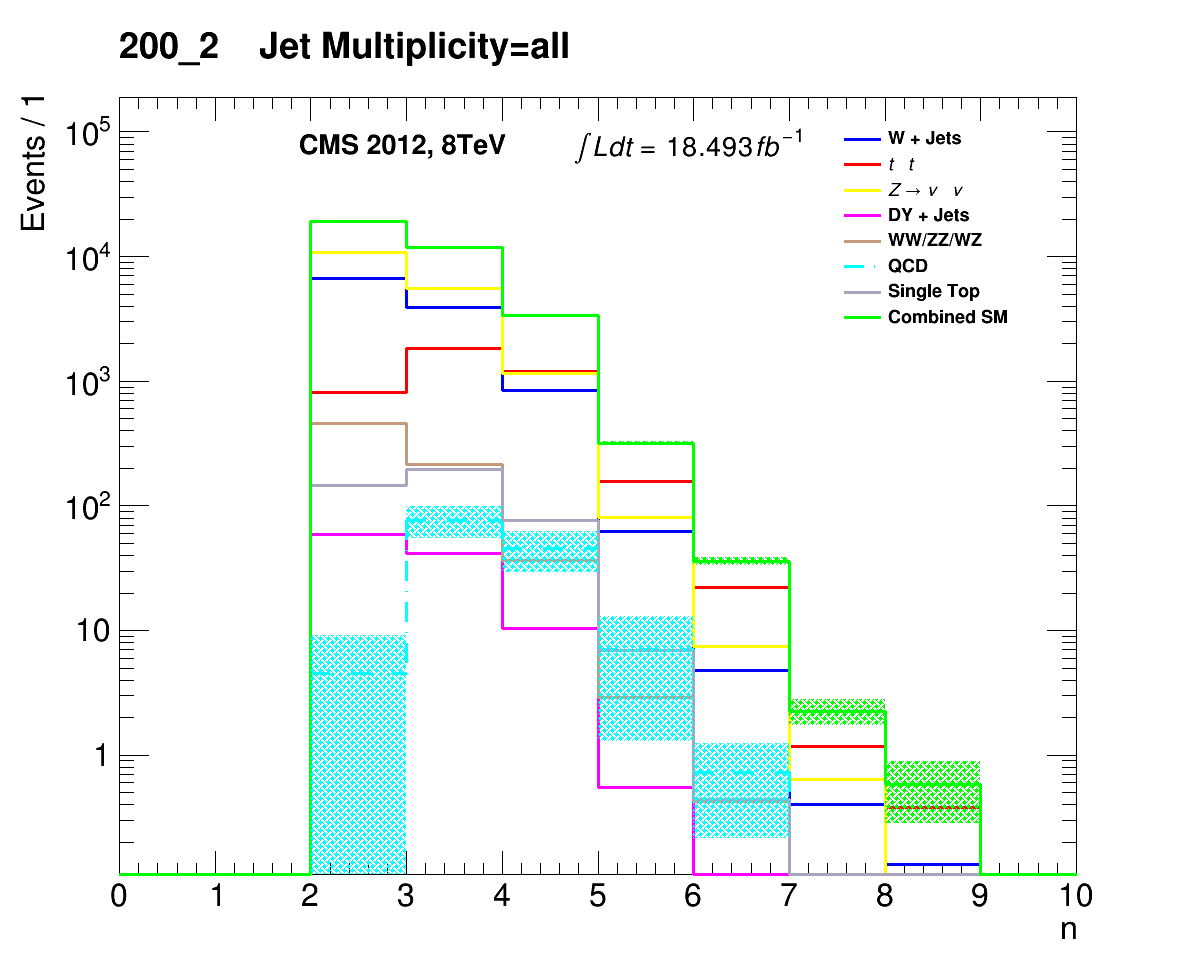
\includegraphics[width=\textwidth]
    {Figs/datamc/had/qcd/JetMultiplicity_all_200_upwards.png}
    \caption{\nj}
    \label{fig:had_qcd_mc_njet}
  \end{subfigure}\\
  \begin{subfigure}[b]{0.46\textwidth}
    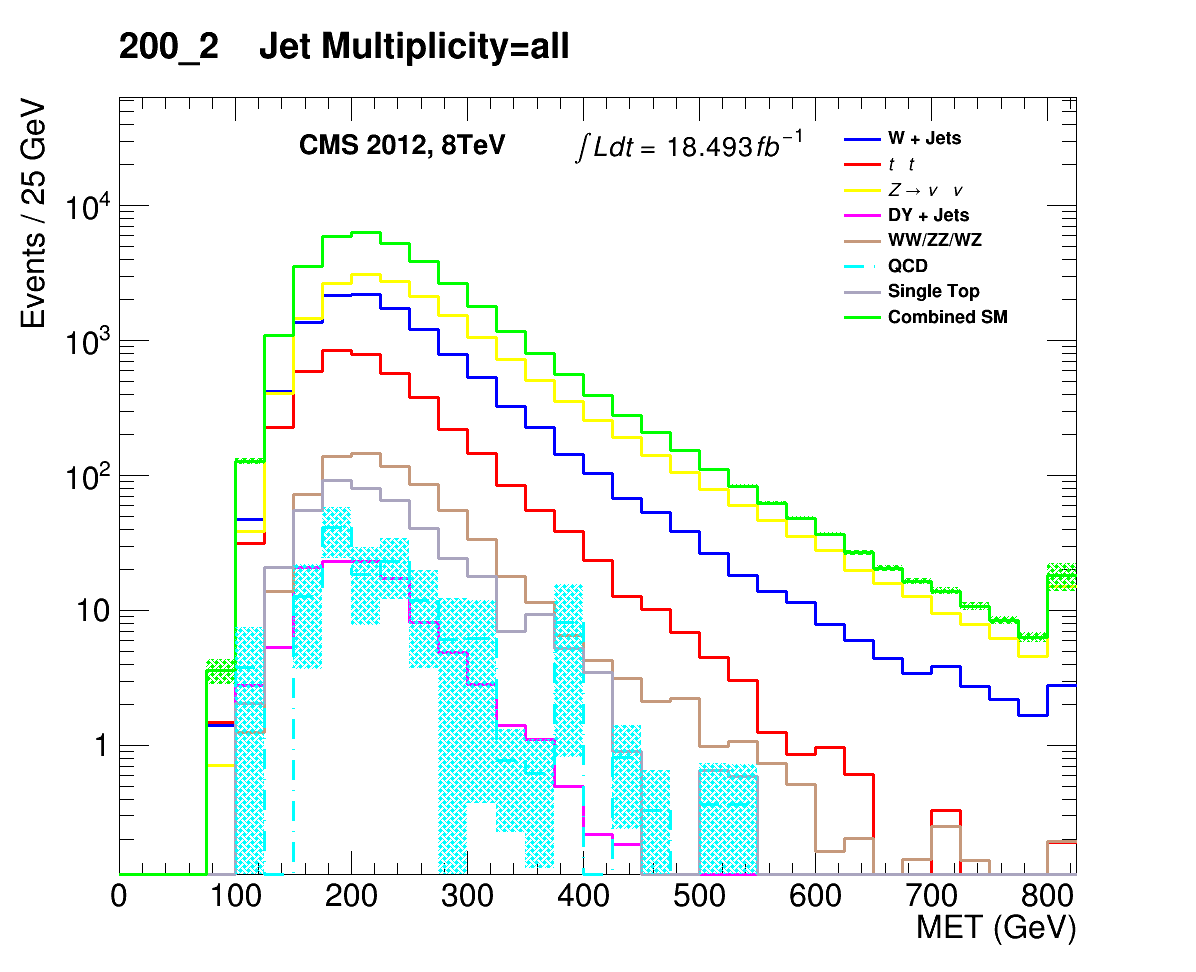
\includegraphics[width=\textwidth]
    {Figs/datamc/had/qcd/MET_all_200_upwards.png}
    \caption{\met}
    \label{fig:had_qcd_mc_met}
  \end{subfigure}
  \begin{subfigure}[b]{0.46\textwidth}
    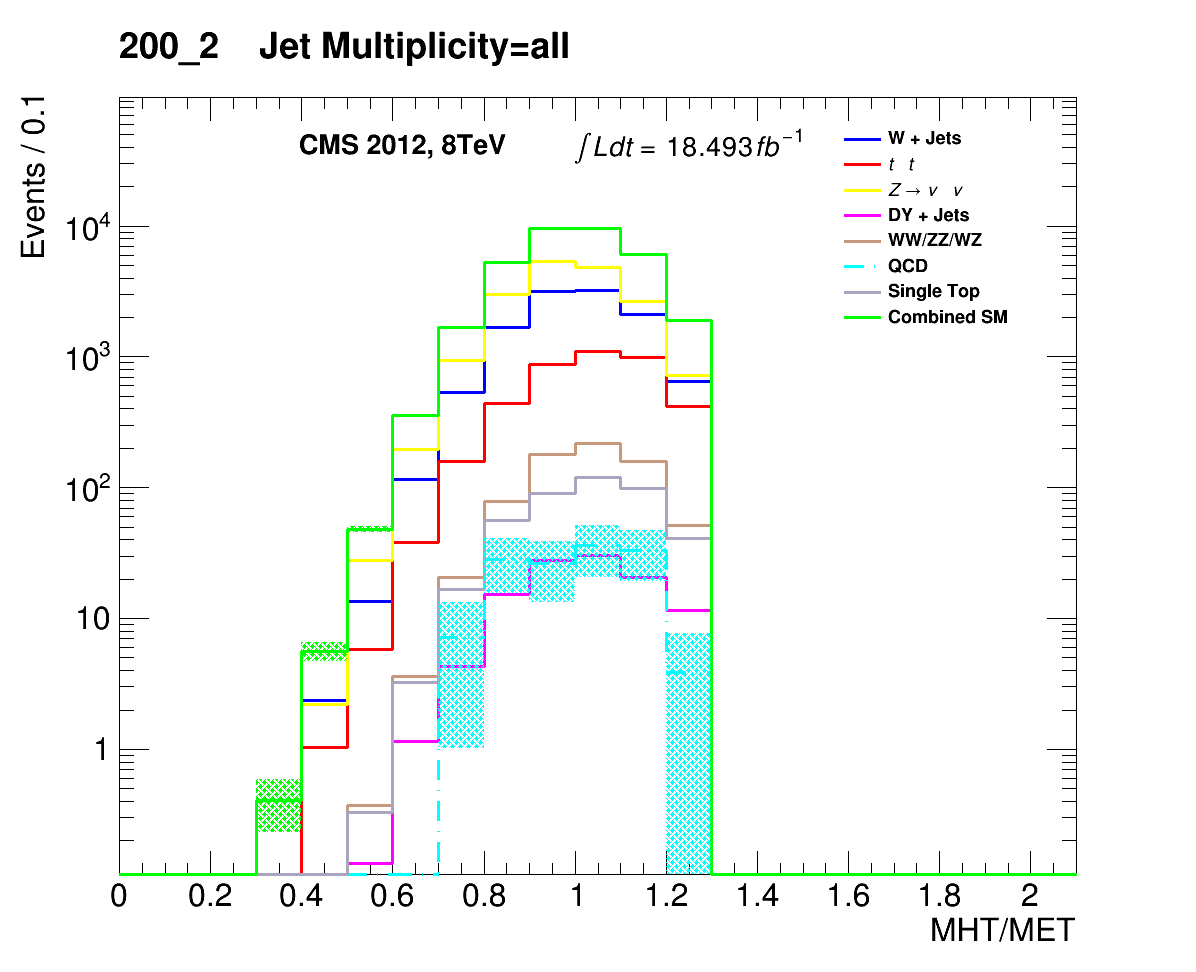
\includegraphics[width=\textwidth]
    {Figs/datamc/had/qcd/MHTovMET_all_200_upwards.png}
    \caption{\mhtmet}
    \label{fig:had_qcd_mc_MHTMET}
  \end{subfigure}
  \caption{Distributions of various event level quantities for simulated MC
  events split by physics process, with QCD shown in cyan. Plots shown are for
  a fully inclusive selection of $\nj\geq2$, $\nb=0$ and $\HT>200\gev$.}
  \label{fig:had_qcd_mc_distros}
\end{figure}

The remaining QCD events contain genuine physics processes, when a jet overlaps
with genuine \met. This missing energy occurs due to heavy flavour mesons in
jets decaying leptonically. Of the lepton and neutrino pair, the neutrino
carries the bulk share of the pair's momentum, leading to soft leptons which
can evade leptonic vetoes and non-negligible amounts of invisible energy. An
event display of a typical event is shown in figure~\ref{fig:event_display_QCD}.
It is important to note the significant amount, 311 \gev, of generator level
\met (`genmetP4True', thin pink arrow) pointing along the axis of a 137
\gev \Pt reconstructed jet (bold blue arrow), a configuration which,
couple with multiple additional jets, can conspire to give
large values of \alphat. The sum of the generator level \met \Pt and
the jet's \Pt sum to the generator level jet's \Pt (bold black arrow),
indicating that the missing energy of the event comes almost entirely from the
neutrinos originating from the jet's decay. Furthermore, this implies the ratio
\mhtmet to be near unity, therefore allowing events to also evade the \mhtmet <
1.25 requirement of the signal region.

\section{Isolating these events}

The variable \mindphistar can be used to isolate these events.

\begin{figure}[h!]
\centering
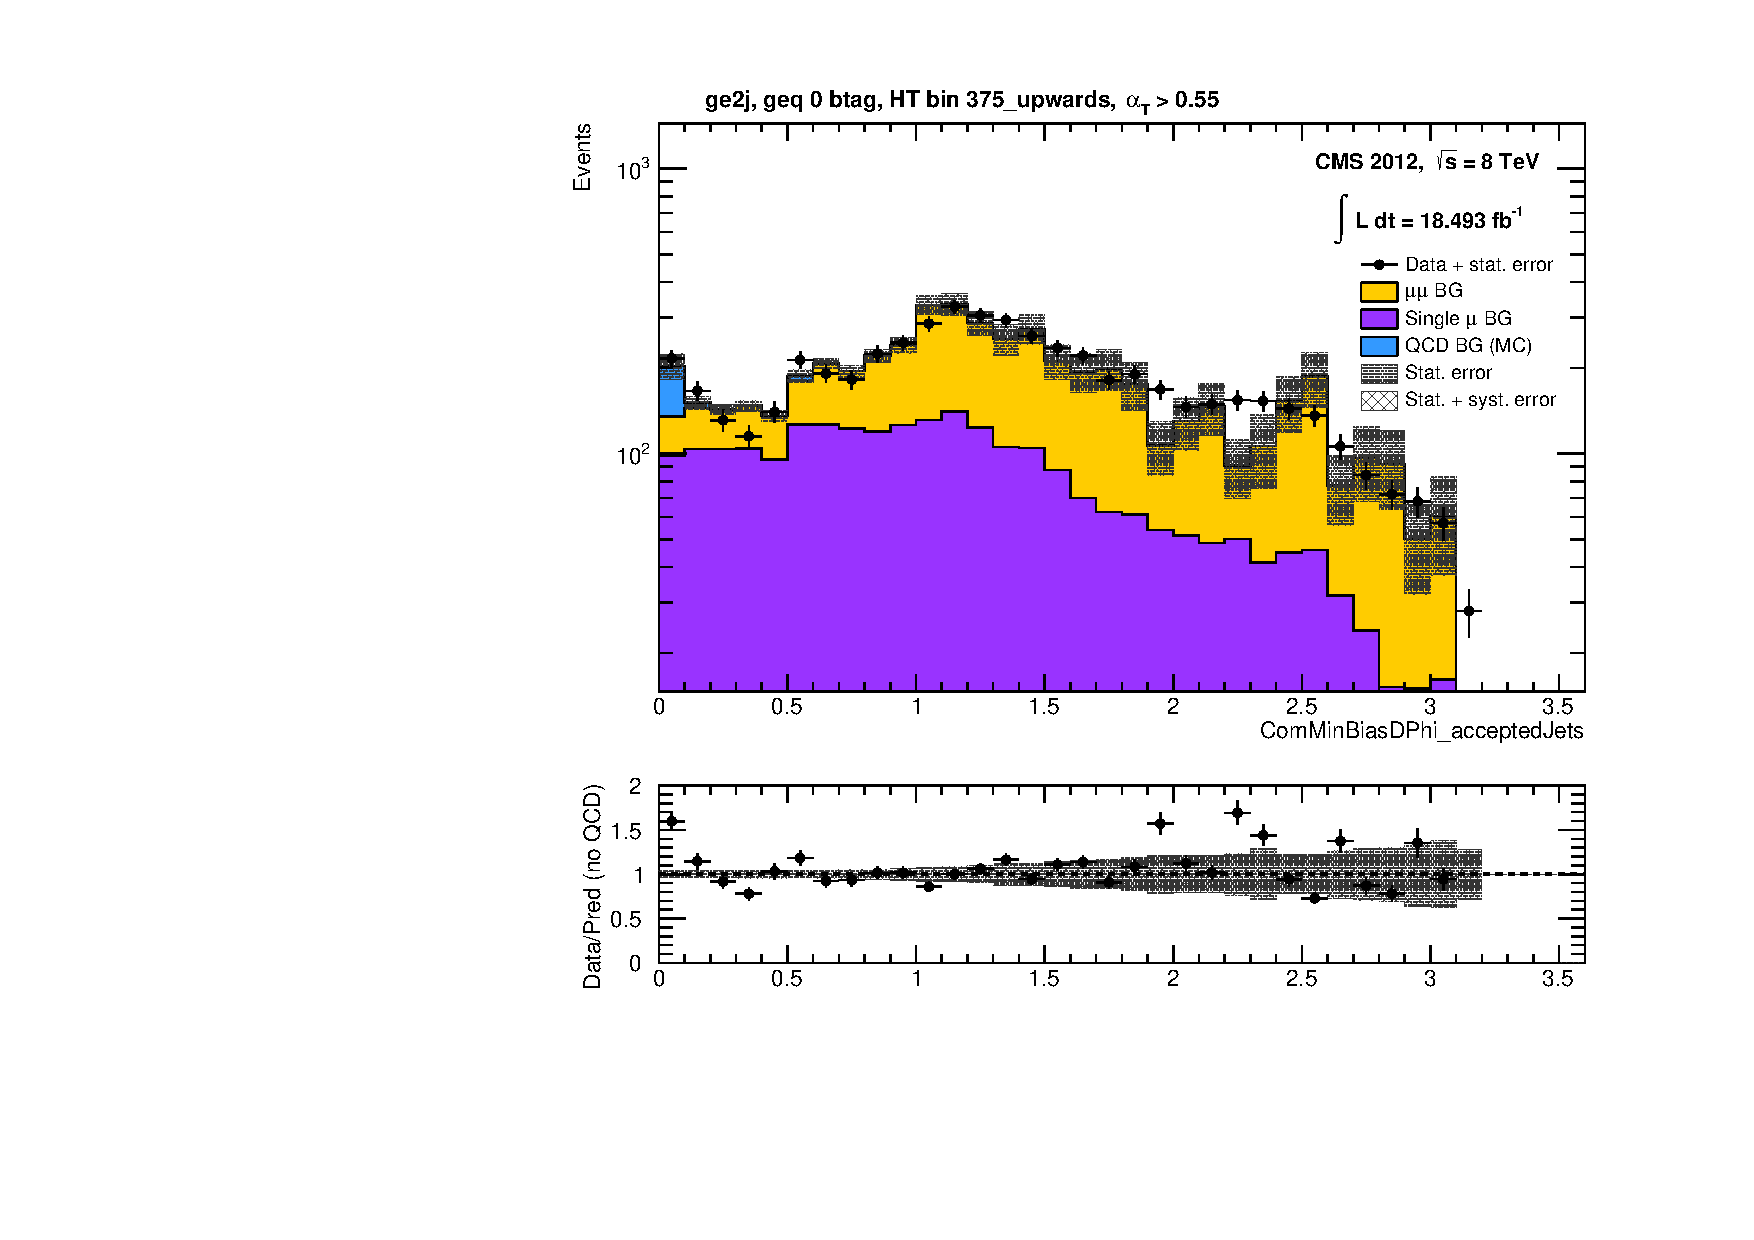
\includegraphics[width=0.5\textwidth]{Figs/datapred/Prediction_ComMinBiasDPhi_acceptedJets_all_375_upwards_QCD.pdf}
\label{fig:data_pred_dphistar_qcd}
\caption{Data}
\end{figure}

It is possible to isolate these events used the \mindphistar variable described
in chapter~\ref{ch:5}. 

can show the QCD MG MC plots of \dphistar - see peak around zero for QCD, even
after full selection and alphaT cuts. Can show without data...! Still though,
what about the handful of events at higher dphistar?

excess vs QCD alphaT evolution plots - observed excess appears to be QCD-like.
\emph{THIS IS ACKNOWLEDGING AN EXCESS!}

\section{Effect of hadronic region}

\emph{How well does this work?} Very well! Removes all remaining QCD events that
contain missing energy. \emph{What about the remaining few QCD MG events at high
dPhiStar?} can show rob's plots of the dphiStar above/below

\section{Effect on signal models}
we do take a hit, but hopefully equivalent of more so in BG pred, so S/B is
preserved. either way, we have to make the cut, so we deal with the consequence
in terms of signal efficiency.

this cut can be particularly damaging to compressed spectra models where a
soft susy decay is balanced by hard ISR, creating co-linear decay products and
neutralino's. ho-hum.

\emph{How much do we `lose' in signal efficiency?} Show signal efficiency
difference plots, with vs without.

\clearpage
\begin{sidewaysfigure}
    \centering
    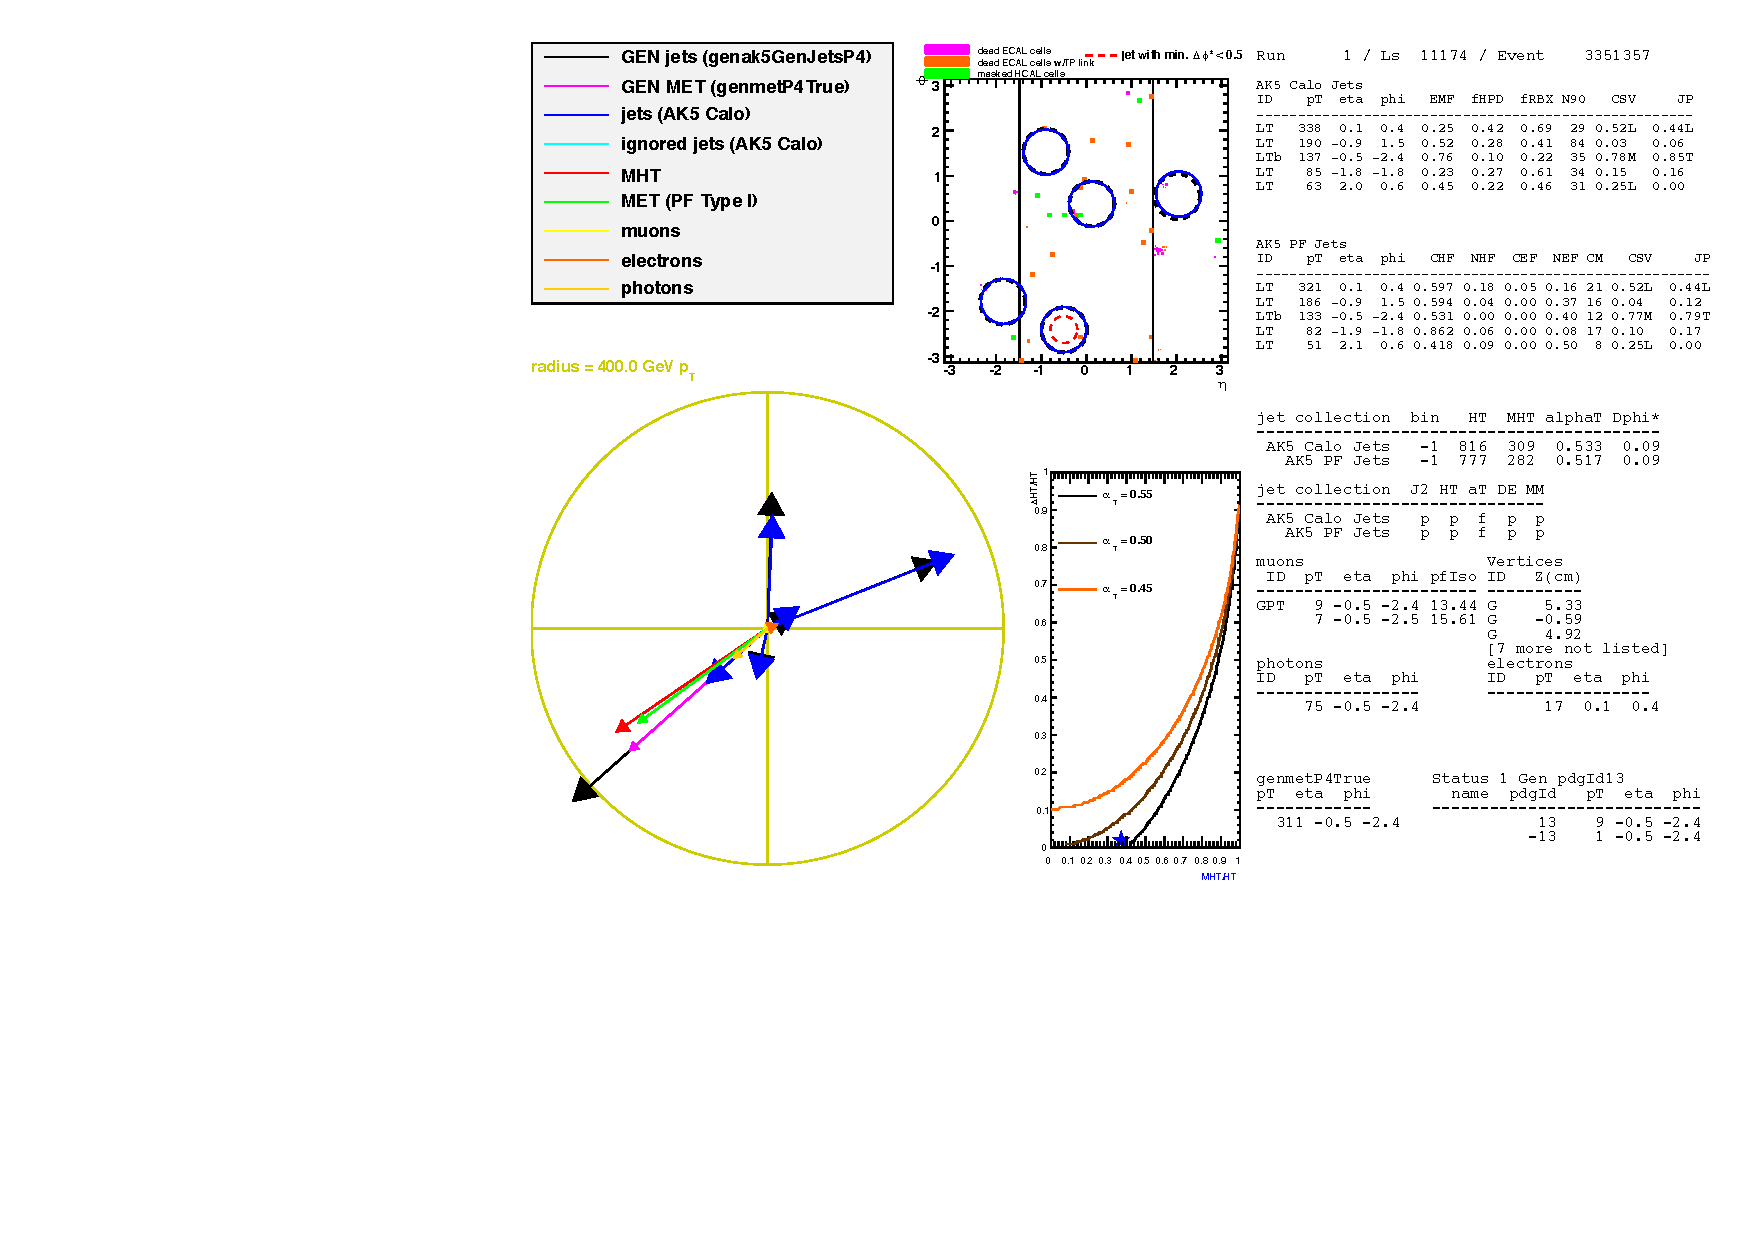
\includegraphics[width=0.95\textwidth]
    {Figs/eventDisplays/Had_QCD_MG_MC_HT375_skim_displays_singleEvent.pdf}
    \caption{Event display blah}
    \label{fig:event_display_QCD}
\end{sidewaysfigure}
